
\section{Overview of Proof Techniques}
\label{sec:sketch}

To avoid notational confusion between discrete-time and continuous-time dynamics, we adopt the following convention throughout this section. Subscripts (e.g., $\W_t$) denote discrete-time quantities, while parentheses (e.g., $\W(t)$) denote continuous-time trajectories. Specifically, $\{\W_t\}_{t \in \mathbb{N}}$ refers to the iterates of online SGD; $\{\W(t)\}_{t \geq 0}$ denotes the continuous-time gradient flow governed by~\eqref{eq:gf}.

Since our proof strategy heavily relies on the matrix (Loewner) order for symmetric matrices, we introduce the following notations. For symmetric matrices $\bs{G}_1, \bs{G}_2 \in \R^{d \times d}$, we write $\bs{G}_1 \prec \bs{G}_2$ (respectively, $\bs{G}_1 \preceq \bs{G}_2$) if $\bs{G}_2 - \bs{G}_1$ is positive definite (respectively, positive semidefinite). The reverse relations are denoted by $\bs{G}_1 \succ \bs{G}_2$ and $\bs{G}_1 \succeq \bs{G}_2$. Figure~\ref{fig:nonmonotone}(a) illustrates this ordering by comparing the level sets of the quadratic forms $\{\bs{v} : \bs{v}^\top \G_i \bs{v} = 1 \}$ for $i = 1, 2$. In particular, $\G_1 \preceq \G_2$ implies that the level sets of $\G_2$ are strictly contained within those of $\G_1$, as shown by the dashed ellipses.

\vspace{-2.5mm}

\subsection{Proof Sketch of Theorem \ref{thm:gfresult}}
\vspace{-0.5mm}
 
 
We first observe that both the population risk $R\big(\W(t)\big)$ and the alignment $\mathrm{Alignment}\big(\W(t), \bs{\theta}_j\big)$ depend on $\W(t)$ through two Gram matrices:  the weight Gram matrix $\G_W(t) \coloneqq \W(t)\W(t)^\top$, and the  alignment Gram matrix $\G_U(t) \coloneqq \Th^\top \U(t)\U(t)^\top \Th$, where $\{\U(t)\}_{t \geq 0}$ denotes the directional component of $\W(t)$, as defined in~\eqref{def:polarcoord}. The proof proceeds by analyzing the evolution of these matrices, each governed by an autonomous ODE; in particular, a matrix Riccati differential equation.   
\begin{proposition}
\label{prop:grammatrixodes}
   The Gram matrices defined above satisfy the following matrix Riccati ODEs:
  \begin{itemize}[leftmargin=*]
      \item  \textbf{Weight Gram matrix:}  $\partial_t \G_{W}(t) = \frac{0.5}{\normL \sqrt{\rs} }   \Big(\Th \bs{\Lambda} \Th^\top  \G_{W}(t)  +  \G_{W}(t) \Th \bs{\Lambda} \Th^\top - \frac{2 \normL}{\sqrt{\rs}}  \G^2_{W}(t) \Big)$.  \vspace{-1mm}
      \item  \textbf{Alignment Gram matrix:} $\partial_t \G_{U}(t) = \frac{0.5}{\normL \sqrt{\rs} } \big(  \bs{\Lambda}    \G_{U}(t)  + \G_{U}(t)  \bs{\Lambda}  - 2  \G_{U}(t)  \bs{\Lambda} \G_{U}(t) \big)$.
  \end{itemize}
\end{proposition}


Both equations in Proposition~\ref{prop:grammatrixodes} take the form of matrix Riccati ODEs~\cite{Bittanti1991TheRE}, whose structural properties play a central role in the proof. To illustrate the core idea, we focus on the alignment dynamics.   For simplicity, we write $\G(t) \coloneqq\G_{U}(t)$  and consider 
\eq{
\partial_t \G(t) =  \frac{0.5}{\normL \sqrt{\rs} }  \left( \bs{\Lambda} \G(t) +    \G(t) \bs{\Lambda}  - 2 \G(t)  \bs{\Lambda} \G(t) \right). \label{eq:contriccati}
}
Note that $\mathrm{Alignment}\big(\W(t), \bs{\theta}_j\big)$ corresponds to the $j$\textsuperscript{th} diagonal entry of $\G(t)$. To characterize its trajectory, we leverage the monotonicity of the matrix Riccati flow with respect to its initialization, i.e., if $\bs{G}_0^+ \! \succeq \! \bs{G}_0^-$,  the corresponding solutions satisfy $\G(t, \bs{G}_0^+) \succeq \G(t, \bs{G}_0^-)$ for all $t \geq 0$, where $\G(t, \bs{G}_0)$ denotes the solution to~\eqref{eq:contriccati} with initial condition $\bs{G}_0$. Our proof strategy builds on this monotonicity and proceeds as follows:
\begin{enumerate}[leftmargin=*,]
\item \textbf{Diagonalization \& decoupling.} If $\G_0$ is diagonal, the solution $\{ \G(t) \}_{t \geq 0}$ remains diagonal under~\eqref{eq:contriccati}, reducing the dynamics to independent scalar ODEs that govern each diagonal entry. Moreover, each scalar ODE admits a closed-form solution, allowing us to track the evolution of individual alignment terms. 
\item \textbf{Asymptotic characterization.} For general $\bs{G}_0$, we construct diagonal matrices $\bs{G}_0^+ \succeq \bs{G}_0 \succeq \bs{G}_0^-$. By monotonicity, the corresponding trajectories upper and lower bound $\{ \G(t) \}_{t \geq 0}$. These bounding systems are diagonal and decoupled, and as $d \to \infty$, their trajectories converge to the same limit.  
\end{enumerate}

We apply this strategy in Appendix \ref{sec:thmgfresult} to derive the exact asymptotics stated in Theorem~\ref{thm:gfresult}.


\begin{remark}
We remark a conceptual point about the monotonicity of Riccati flow: {while the Riccati flow is monotone with respect to its initialization, this does not imply that its solution is monotone in time.} That is, the trajectory $\G(t)$ may not evolve monotonically in matrix order, even though a larger initialization yields a trajectory that remains above that of a smaller one for all $t \geq 0$. This distinction is illustrated in Figure~\ref{fig:nonmonotone}.
\end{remark}

 
\begin{figure}[t]
% \vspace{-2mm}
    \centering
    \begin{subfigure}[t]{0.48\textwidth}
        \centering
        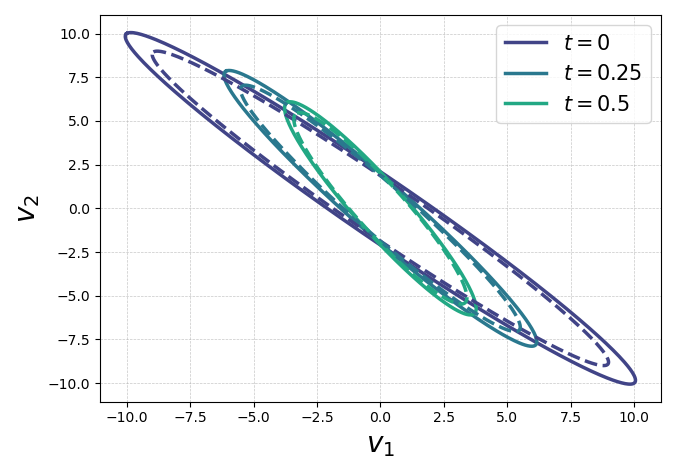
\includegraphics[width=0.9\textwidth]{_figures/twodimensional.png}
        \vspace{-2mm}
        \caption{Trajectory in matrix order.}
    \end{subfigure} 
    \begin{subfigure}[t]{0.48\textwidth}
        \centering
        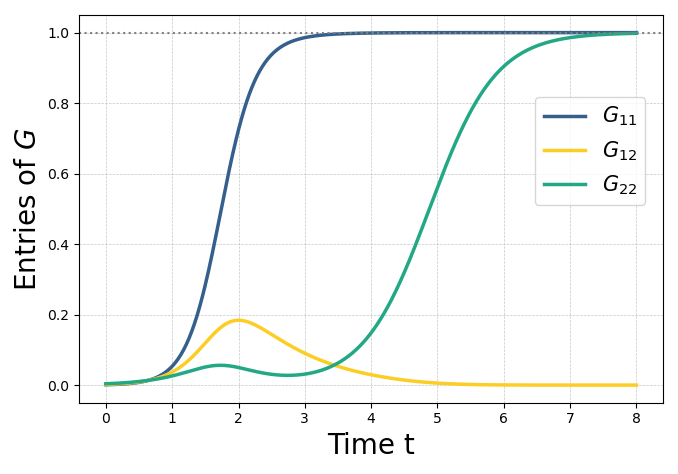
\includegraphics[width=0.9\textwidth]{_figures/entriesofG.png}
        \vspace{-2mm}
        \caption{Trajectory of entries of the Gram matrix.}
    \end{subfigure} 
\caption{\small Solutions of the matrix Riccati ODE in \eqref{eq:contriccati} with $\lambda_1 = 2$, $\lambda_2 = 1$, $\rs = 2$.
\emph{(a)} To visualize the dynamics under matrix order, we plot the level sets of $\G(t)$ at times $t \in \{0, 0.25, 0.5\}$ for two initializations: $\G(0)$ (solid) and a scaled version $1.25\,\G(0)$ (dashed). The dashed ellipses remain enclosed within the solid ones at all times, illustrating monotonicity of the Riccati flow \textit{with respect to initialization}. However, note that $\G(t)$ is not monotone in Loewner order over time, as seen from the lack of nesting among the solid ellipses. 
\emph{(b)} Entry-wise evolution of $\G(t)$ under a random initialization with $d = 1024$. The diagonal entry $\G_{22}(t)$ exhibits non-monotonic behavior, illustrating that the solution trajectory $\G(t)$ need not be monotone in time; the off-diagonal entry $\G_{12}(t)$ is also shown for reference.}
\label{fig:nonmonotone}
% \vspace{-1em}
\end{figure}
 
\subsection{Proof Sketch of Theorem \ref{thm:sgdresult}}
\subsubsection*{Extending Monotonicity Arguments to Discrete Dynamics}

We begin by observing that online SGD on the Stiefel manifold approximates the directional component of the continuous-time gradient flow, with stochastic gradients arising from online sampling. This connection becomes apparent when comparing the discrete and continuous dynamics:
\begin{alignat}{2}
\hspace{-2.4em} \textbf{SGD on Stiefel:} ~~~
& \bs{\widetilde{W}}_{t} = \bs{W}_{t-1} - \eta \nabla_{\mathrm{St}} \mathcal{L}(\bs{W}_{t-1}) \quad \Rightarrow \quad
&& \textbf{GF on Stiefel:} ~~~
  \partial_t \widehat{\W}(t) = -\nabla_{\mathrm{St}} R\big( \widehat{\W}(t) \big).   \label{eq:continousdirectional} \\
& \bs{W}_{t} = \bs{\widetilde{W}}_{t} \left( \bs{\widetilde{W}}_{t}^\top \bs{\widetilde{W}}_{t} \right)^{-1/2}
\ && 
\end{alignat}
The proposition below formalizes the idea that online SGD approximates the directional dynamics of the continuous gradient flow at the population level. For the statement, recall that $\bs{U}(t)$ denotes the directional component of the gradient flow solution $\bs{W}(t)$ from \eqref{eq:gf}, as defined in \eqref{def:polarcoord}. 
\begin{proposition}
\label{prop:sgdrotation}
Let $\widehat{\bs{W}}(t)$ be the solution to the continuous-time gradient flow on the Stiefel manifold defined in \eqref{eq:continousdirectional}, initialized with $\bs{U}(0)$. Then for all $t \geq 0$, the column spaces of $\widehat{\bs{W}}(t)$ and $\bs{U}(t)$ coincide.
\end{proposition}

This result justifies studying the online SGD on Steifel manifold via the directional dynamics of \eqref{eq:gf}.
 To this end, we introduce the discrete analog of $\G(t)$ above as $\G_t = \Th^\top \W_t \W_t^\top \Th$. Extending the analysis to discrete time is non-trivial due to the \emph{loss of monotonicity} in the Euler discretization of the Riccati dynamics~\eqref{eq:contriccati}. In particular, the update
\eq{
\underbrace{ 
\G_{t} = \G_{t-1} + \tfrac{0.5 \eta}{\normL \sqrt{\rs}} \left(  \bs{\Lambda} \G_{t-1} + \G_{t-1}\bs{\Lambda}  - 2 \G_{t-1} \bs{\Lambda}  \G_{t-1}\right)   }_{\text{non-monotone dynamics}}
+ ~\text{(2nd-order terms and noise)}   \hspace{1.2em}
\label{eq:gndiscrete}
}
no longer preserves the matrix order structure crucial to the continuous-time argument.

To overcome this, we construct an auxiliary discrete system that approximates~\eqref{eq:gndiscrete} up to second-order terms while preserving monotonicity. Specifically, we define the map
\eq{
\G(\G_t ,\eta)   \coloneqq    \bs{G}_t   -  \frac{\eta}{2} (2 \bs{G}_t - \bs{I}_r) \bs{\Lambda}  (2 \bs{G}_t - \bs{I}_r)  \left(   \bs{I}_r \! + \!  \eta \bs{\Lambda} (2 \bs{G}_t - \bs{I}_r )   \right)^{-1}   +   \eta \bs{\Lambda} \hspace{1em}\label{eq:gdnricc}
}
which matches~\eqref{eq:gndiscrete} up to second-order terms. Indeed, expanding the inverse term gives 
\eq{
\textstyle
\G(\G_t , \eta)  & = \underbrace{ \bs{G}_t  - \frac{\eta}{2}  (2 \bs{G}_t - \bs{I}_r) \bs{\Lambda}  (2 \bs{G}_t - \bs{I}_r) + \eta \bs{\Lambda} }_{  = \bs{G}_t +  \eta \left(  \bs{\Lambda} \bs{G}_t + \bs{G}_t\bs{\Lambda}  - 2 \bs{G}_t \bs{\Lambda}  \bs{G}_t\right) } + ~ \text{2nd-order terms}.
}
The key advantage of the iteration~\eqref{eq:gdnricc} is that it preserves matrix order:
\begin{proposition}
\label{prop:monotoneupdatetext}
    For $  \eta > 0$, if $\bs{G}^{+}_t \succeq \bs{G}^{-}_t \succeq 0$, we have   $\G(\G^+_t, \eta) \succeq \G(\G^-_t, \eta)$.
\end{proposition}
We use this to bound the non-monotone dynamics~\eqref{eq:gndiscrete} via monotone iterates. Roughly,  we show that for small enough step size 
$\eta$,  the following holds: 
\eq{
\G \big(\G_{t-1},   (1 + \varepsilon) \lr \big) +  \text{ Noise}   \succeq  \bs{G}_{t}   \succeq  \G \big(\G_{t-1},  (1 - \varepsilon) \lr \big) +   \text{ Noise}  \label{eq:boundingdiscrete} 
}
for some $\varepsilon = o_d(1)$,  where we denote the effective learning rate in~\eqref{eq:gndiscrete} with $\lr = \tfrac{\eta}{\sqrt{\rs} \normL}$.  We then follow the same bounding argument used in the continuous case by defining the upper and lower reference sequences, 
\eq{
\G_{t}^\pm  = \G \big(\G^{\pm}_{t-1},  (1 \pm \varepsilon)\lr \big) + \text{Noise}, ~~ \text{where} ~~ \G_0^+ \succeq \G_0 \succeq \G_0^- \succeq 0,
}
show that $\G_t^+ \succeq \G_t \succeq \G_t^-$ for all $t \in \N$.
Finally, by choosing $\G^{\pm}_0$ to be diagonal, the bounding dynamics reduce to decoupled scalar recursions, which can be analyzed explicitly. This allows us to establish concentration of the original iterates $\{ \G_{t} \}_{t \in \N}$ around the bounding sequences, leading to operator-norm convergence of the discrete-time dynamics to their continuous-time counterparts. See Appendix~\ref{sec:defs} for full argument.

\subsubsection*{Risk Decomposition for Fine Tuning}

The fine-tuning step relies on the following decomposition of the population risk:

\begin{proposition}
\label{prop:riskdecomptext}
    For any $\bs{\Omega} \in \R^{\rs \times \rs}$, the population risk defined in \eqref{eq:poprisk} can be written as:
    \eq{
R(\W_t \bs{\Omega}) =  \frac{1}{\rs}  \norm*{ \bs{\Omega} \bs{\Omega}^\top - \tfrac{\sqrt{\rs}}{\normL}  \W_t^\top \Th \bs{\Lambda} \Th^\top \W_t }_F^2 + \frac{1}{\normL^2} \Big( \normL^2 -   \norm{\bs{\Lambda}^{\frac{1}{2}}  \G_t \bs{\Lambda}^{\frac{1}{2}}}_F^2   \Big) ,
}
where  $\G_t = \Th^\top \W_t \W_t^\top \Th$ is the discrete alignment Gram matrix defined in the previous part.
\end{proposition}

We observe  that both the second term and the matrix $\bs{W}_t^\top \bs{\Theta} \bs{\Lambda} \bs{\Theta}^\top \bs{W}_t$ are independent of $\bs{\Omega}$. Hence, the fine-tuning step reduces to a least squares problem in the matrix $\bs{\Omega} \bs{\Omega}^\top$ in population, which is approximated via empirical risk minimization over a fresh batch of samples. By standard concentration arguments, a sample size of $N_{\mathrm{Ft}} \geq \rs^2 \mathrm{polylog} d$ suffices to ensure that the empirical minimizer approximates the population solution with high probability. Full details are provided in Appendix~\ref{sec:finetuning}.
